\section{Results and Discussion}

In order to broadly assess the selective consequences of each treatment with respect to the functional and reproductive cooperation characteristic of evolutionary transitions of individuality, we begin with aggregate analysis of the relationship between same-channel signaling network context and resource-sharing and cell reproduction behavior.
Then, in section \ref{sec:life-cycles} we will survey observed multicellular life cycles.

Subsequent sections describe the mechanistic underpinnings and fitness effects of notable phenotypic traits that evolved in individual replicates.
Section \ref{sec:gene-regulation} reports an endogenous propagule-seeding strategy mediated by gene regulation.
Section \ref{sec:gradient-conditioned-behavior} describes cell behavior plastically conditioned by a resource gradient.
Section \ref{sec:morphology} details a stringy same-channel signaling network morphology.
Section \ref{sec:cell-cell-messaging} provides two examples of adaptive cell-cell messaging.
Finally, section \ref{sec:apoptosis} reviews two replicates where widespread apoptosis evolved.

\begin{figure*}[!htbp]
\begin{center}

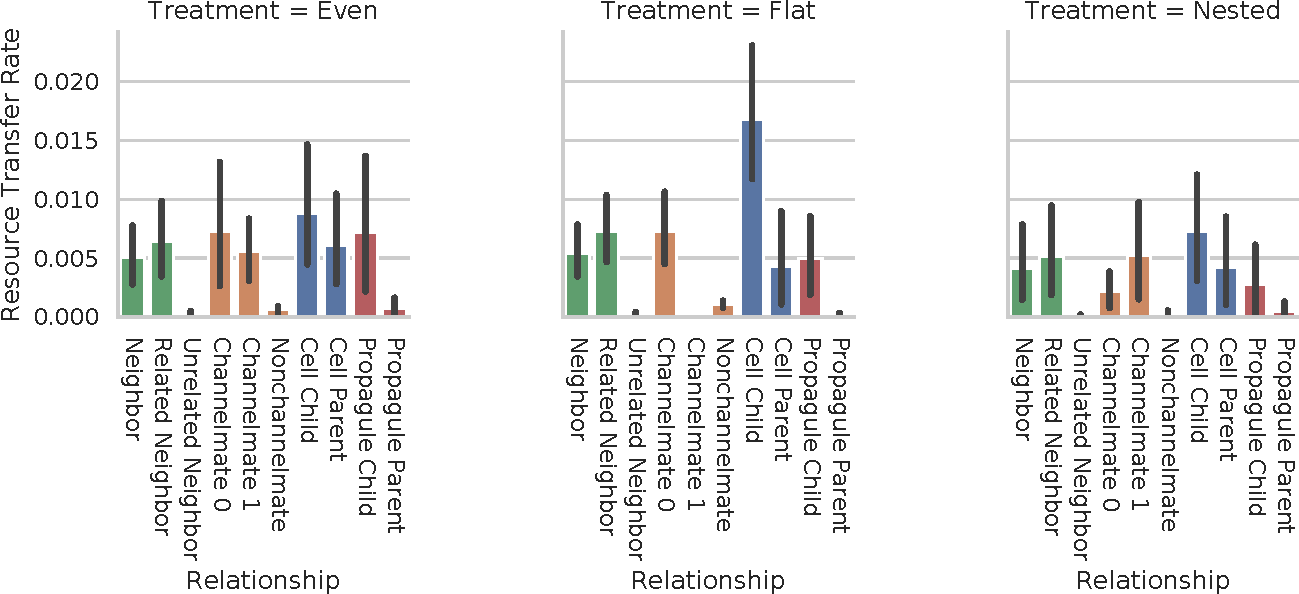
\includegraphics[width=\textwidth]{sharing/title=Resource_Transfer_Rate+_data_hathash_hash=e07865a0aee42cf7+_script_fullcat_hash=3612aad527ec4368+_source_hash=ffbe01c-clean+ext=}

\caption{
TODO
}
\label{fig:sharing}
\end{center}
\end{figure*}


\subsection{Reproductive Cooperation}

\begin{figure*}[!htbp]
\begin{center}
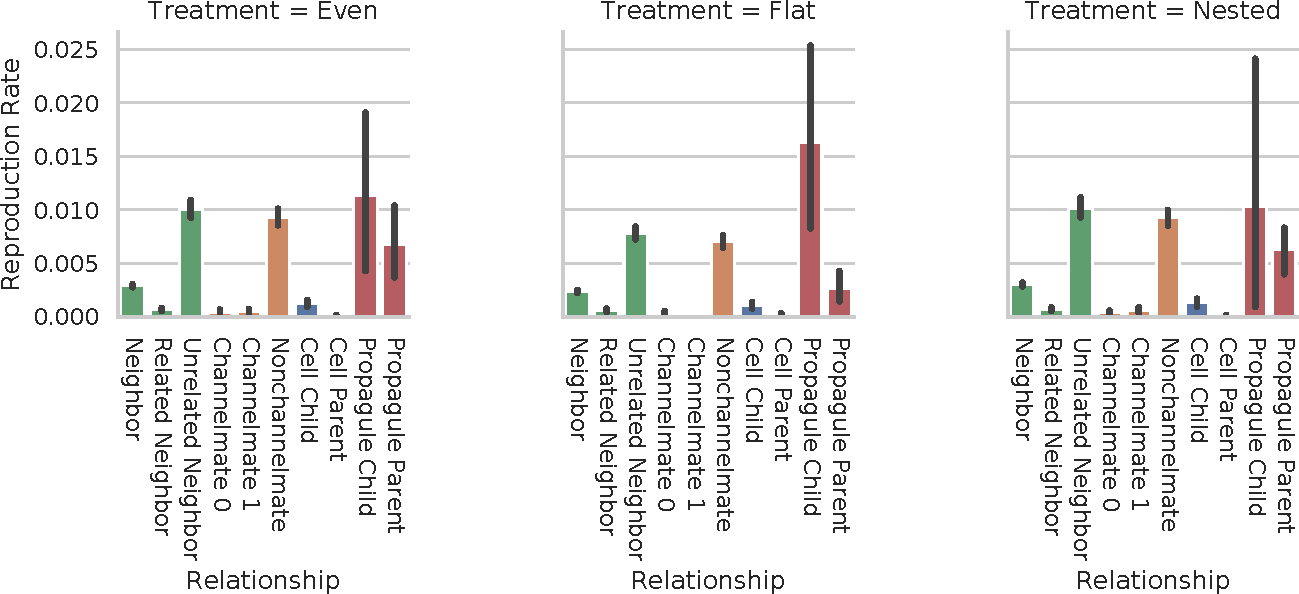
\includegraphics[width=\textwidth]{reproduction/title=Reproduction_Rate+_data_hathash_hash=abbd7dbb4cba6da1+_script_fullcat_hash=3612aad527ec4368+_source_hash=ffbe01c-clean+ext=}
\includegraphics[width=\textwidth]{reproduction_corrupt/title=Reproduction_Rate+_data_hathash_hash=fba4429b39fb0e53+_script_fullcat_hash=3612aad527ec4368+_source_hash=ffbe01c-clean+ext=}
\caption{
TODO
}
\label{fig:reproduction}
\end{center}
\end{figure*}


\begin{figure}[!htbp]
\begin{center}

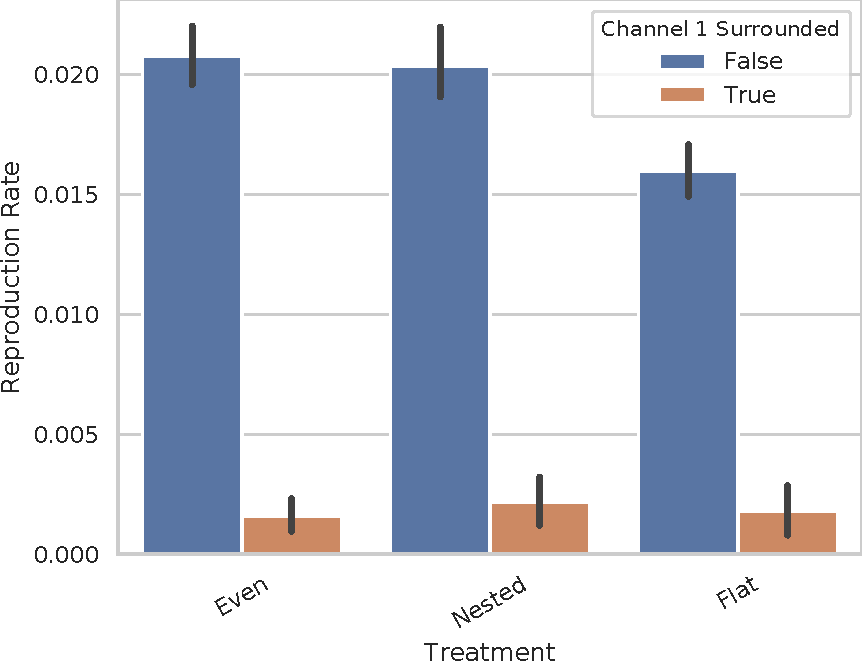
\includegraphics[width=\columnwidth]{reproduction/title=reproductive_labor_surrounded+_data_hathash_hash=4e1be4c5abfa4b05+_script_fullcat_hash=62ec0af515e8429d+_source_hash=ffbe01c-clean+ext=}

\caption{
TODO
}
\label{fig:reproduction_surrounted}
\end{center}
\end{figure}


\subsection{Propagule Generation}

\begin{figure*}[!htbp]
\begin{center}

\begin{subfigure}[b]{\textwidth}
\centering
\begin{minipage}[t]{0.18\textwidth}
\centering
\adjincludegraphics[width=\textwidth, trim={{.66\width} {.66\width} {.0\width} {.0\width}}, clip]{lifecycle/transfer-paint/seed=1004+title=directional_propagule_viz+treat=resource-wave__channelsense-yes__nlev-two+update=1048896+_data_hathash_hash=06a65518d5588ef3+_script_fullcat_hash=8b1f57a580a67198+_source_hash=ffbe01c-clean+ext=}
Update 0
\end{minipage}
\begin{minipage}[t]{0.18\textwidth}
\centering
\adjincludegraphics[width=\textwidth, trim={{.66\width} {.66\width} {.0\width} {.0\width}}, clip]{lifecycle/transfer-paint/seed=1004+title=directional_propagule_viz+treat=resource-wave__channelsense-yes__nlev-two+update=1048928+_data_hathash_hash=06a65518d5588ef3+_script_fullcat_hash=8b1f57a580a67198+_source_hash=ffbe01c-clean+ext=}
Update 32
\end{minipage}
\begin{minipage}[t]{0.18\textwidth}
\centering
\adjincludegraphics[width=\textwidth, trim={{.66\width} {.66\width} {.0\width} {.0\width}}, clip]{lifecycle/transfer-paint/seed=1004+title=directional_propagule_viz+treat=resource-wave__channelsense-yes__nlev-two+update=1048960+_data_hathash_hash=06a65518d5588ef3+_script_fullcat_hash=8b1f57a580a67198+_source_hash=ffbe01c-clean+ext=}
Update 64
\end{minipage}
\begin{minipage}[t]{0.18\textwidth}
\centering
\adjincludegraphics[width=\textwidth, trim={{.66\width} {.66\width} {.0\width} {.0\width}}, clip]{lifecycle/transfer-paint/seed=1004+title=directional_propagule_viz+treat=resource-wave__channelsense-yes__nlev-two+update=1049024+_data_hathash_hash=06a65518d5588ef3+_script_fullcat_hash=8b1f57a580a67198+_source_hash=ffbe01c-clean+ext=}
Update 128
\end{minipage}
\begin{minipage}[t]{0.18\textwidth}
\centering
\adjincludegraphics[width=\textwidth, trim={{.66\width} {.66\width} {.0\width} {.0\width}}, clip]{lifecycle/transfer-paint/seed=1004+title=directional_propagule_viz+treat=resource-wave__channelsense-yes__nlev-two+update=1049408+_data_hathash_hash=06a65518d5588ef3+_script_fullcat_hash=8b1f57a580a67198+_source_hash=ffbe01c-clean+ext=}
Update 512
\end{minipage}
\caption{Spawn TODO}
\label{fig:TODO}
\end{subfigure}

\vspace{3ex}

\begin{subfigure}[b]{\textwidth}
\centering
\begin{minipage}[t]{0.18\textwidth}
\centering
\adjincludegraphics[width=\textwidth, trim={{.0\width} {.0\width} {.66\width} {.66\width}}, clip]{lifecycle/replace-paint/seed=1023+title=directional_propagule_viz+treat=resource-wave__channelsense-yes__nlev-two+update=1048576+_data_hathash_hash=39aa6b64134daefa+_script_fullcat_hash=8b1f57a580a67198+_source_hash=ffbe01c-clean+ext=}
Update 0
\end{minipage}
\begin{minipage}[t]{0.18\textwidth}
\centering
\adjincludegraphics[width=\textwidth, trim={{.0\width} {.0\width} {.66\width} {.66\width}}, clip]{lifecycle/replace-paint/seed=1023+title=directional_propagule_viz+treat=resource-wave__channelsense-yes__nlev-two+update=1048648+_data_hathash_hash=39aa6b64134daefa+_script_fullcat_hash=8b1f57a580a67198+_source_hash=ffbe01c-clean+ext=}
Update 72
\end{minipage}
\begin{minipage}[t]{0.18\textwidth}
\centering
\adjincludegraphics[width=\textwidth, trim={{.0\width} {.0\width} {.66\width} {.66\width}}, clip]{lifecycle/replace-paint/seed=1023+title=directional_propagule_viz+treat=resource-wave__channelsense-yes__nlev-two+update=1048720+_data_hathash_hash=39aa6b64134daefa+_script_fullcat_hash=8b1f57a580a67198+_source_hash=ffbe01c-clean+ext=}
Update 144
\end{minipage}
\begin{minipage}[t]{0.18\textwidth}
\centering
\adjincludegraphics[width=\textwidth, trim={{.0\width} {.0\width} {.66\width} {.66\width}}, clip]{lifecycle/replace-paint/seed=1023+title=directional_propagule_viz+treat=resource-wave__channelsense-yes__nlev-two+update=1048792+_data_hathash_hash=39aa6b64134daefa+_script_fullcat_hash=8b1f57a580a67198+_source_hash=ffbe01c-clean+ext=}
Update 216
\end{minipage}
\begin{minipage}[t]{0.18\textwidth}
\centering
\adjincludegraphics[width=\textwidth, trim={{.0\width} {.0\width} {.66\width} {.66\width}}, clip]{lifecycle/replace-paint/seed=1023+title=directional_propagule_viz+treat=resource-wave__channelsense-yes__nlev-two+update=1048864+_data_hathash_hash=39aa6b64134daefa+_script_fullcat_hash=8b1f57a580a67198+_source_hash=ffbe01c-clean+ext=}
Update 288
\end{minipage}
\caption{Replace TODO}
\label{fig:TODO}
\end{subfigure}

\vspace{3ex}

\begin{subfigure}[b]{\textwidth}
\centering
\begin{minipage}[t]{0.18\textwidth}
\centering
\adjincludegraphics[width=\textwidth, trim={{.0\width} {.66\width} {.66\width} {.0\width}}, clip]{lifecycle/burst-paint/seed=1034+title=directional_propagule_viz+treat=resource-wave__channelsense-yes__nlev-two+update=1048648+_data_hathash_hash=02a94757e9b17a36+_script_fullcat_hash=8b1f57a580a67198+_source_hash=ffbe01c-clean+ext=}
Update 0
\end{minipage}
\begin{minipage}[t]{0.18\textwidth}
\centering
\adjincludegraphics[width=\textwidth, trim={{.0\width} {.66\width} {.66\width} {.0\width}}, clip]{lifecycle/burst-paint/seed=1034+title=directional_propagule_viz+treat=resource-wave__channelsense-yes__nlev-two+update=1048744+_data_hathash_hash=02a94757e9b17a36+_script_fullcat_hash=8b1f57a580a67198+_source_hash=ffbe01c-clean+ext=}
Update 96
\end{minipage}
\begin{minipage}[t]{0.18\textwidth}
\centering
\adjincludegraphics[width=\textwidth, trim={{.0\width} {.66\width} {.66\width} {.0\width}}, clip]{lifecycle/burst-paint/seed=1034+title=directional_propagule_viz+treat=resource-wave__channelsense-yes__nlev-two+update=1048840+_data_hathash_hash=02a94757e9b17a36+_script_fullcat_hash=8b1f57a580a67198+_source_hash=ffbe01c-clean+ext=}
Update 192
\end{minipage}
\begin{minipage}[t]{0.18\textwidth}
\centering
\adjincludegraphics[width=\textwidth, trim={{.0\width} {.66\width} {.66\width} {.0\width}}, clip]{lifecycle/burst-paint/seed=1034+title=directional_propagule_viz+treat=resource-wave__channelsense-yes__nlev-two+update=1048936+_data_hathash_hash=02a94757e9b17a36+_script_fullcat_hash=8b1f57a580a67198+_source_hash=ffbe01c-clean+ext=}
Update 288
\end{minipage}
\begin{minipage}[t]{0.18\textwidth}
\centering
\adjincludegraphics[width=\textwidth, trim={{.0\width} {.66\width} {.66\width} {.0\width}}, clip]{lifecycle/burst-paint/seed=1034+title=directional_propagule_viz+treat=resource-wave__channelsense-yes__nlev-two+update=1049032+_data_hathash_hash=02a94757e9b17a36+_script_fullcat_hash=8b1f57a580a67198+_source_hash=ffbe01c-clean+ext=}
Update 384
\end{minipage}
\caption{Burst TODO}
\label{fig:TODO}
\end{subfigure}

\vspace{3ex}

\begin{subfigure}[b]{\textwidth}
\centering
\begin{minipage}[t]{0.18\textwidth}
\centering
\adjincludegraphics[width=\textwidth, trim={{.5\width} {.33\width} {.17\width} {.33\width}}, clip]{lifecycle/cell-paint/seed=1026+title=directional_daughter_viz+treat=resource-wave__channelsense-yes__nlev-two+update=1048576+_data_hathash_hash=a22f7463ee6886d7+_script_fullcat_hash=ef865c98cd111636+_source_hash=ffbe01c-clean+ext=}
Update 0
\end{minipage}
\begin{minipage}[t]{0.18\textwidth}
\centering
\adjincludegraphics[width=\textwidth, trim={{.5\width} {.33\width} {.17\width} {.33\width}}, clip]{lifecycle/cell-paint/seed=1026+title=directional_daughter_viz+treat=resource-wave__channelsense-yes__nlev-two+update=1048704+_data_hathash_hash=a22f7463ee6886d7+_script_fullcat_hash=ef865c98cd111636+_source_hash=ffbe01c-clean+ext=}
Update 128
\end{minipage}
\begin{minipage}[t]{0.18\textwidth}
\centering
\adjincludegraphics[width=\textwidth, trim={{.5\width} {.33\width} {.17\width} {.33\width}}, clip]{lifecycle/cell-paint/seed=1026+title=directional_daughter_viz+treat=resource-wave__channelsense-yes__nlev-two+update=1048832+_data_hathash_hash=a22f7463ee6886d7+_script_fullcat_hash=ef865c98cd111636+_source_hash=ffbe01c-clean+ext=}
Update 256
\end{minipage}
\begin{minipage}[t]{0.18\textwidth}
\centering
\adjincludegraphics[width=\textwidth, trim={{.5\width} {.33\width} {.17\width} {.33\width}}, clip]{lifecycle/cell-paint/seed=1026+title=directional_daughter_viz+treat=resource-wave__channelsense-yes__nlev-two+update=1048960+_data_hathash_hash=a22f7463ee6886d7+_script_fullcat_hash=ef865c98cd111636+_source_hash=ffbe01c-clean+ext=}
Update 384
\end{minipage}
\begin{minipage}[t]{0.18\textwidth}
\centering
\adjincludegraphics[width=\textwidth, trim={{.5\width} {.33\width} {.17\width} {.33\width}}, clip]{lifecycle/cell-paint/seed=1026+title=directional_daughter_viz+treat=resource-wave__channelsense-yes__nlev-two+update=1049088+_data_hathash_hash=a22f7463ee6886d7+_script_fullcat_hash=ef865c98cd111636+_source_hash=ffbe01c-clean+ext=}
Update 512
\end{minipage}
\caption{Cellular TODO}
\label{fig:TODO}
\end{subfigure}


\caption{
TODO
same-channel signaling networks
}
\label{fig:ko-apoptosis}
\end{center}
\end{figure*}


\subsection{Case Study: Apoptosis}

\begin{figure}[!htbp]
\begin{center}

\hspace*{\fill}%
\begin{minipage}[t]{0.05\columnwidth}
\vspace{0pt} % for alignment
\rotatebox{90}{Strain A}%
\end{minipage}%
\hfill
\begin{minipage}[t]{0.45\columnwidth}
\centering
\vspace{0pt} % for alignment
\adjincludegraphics[width=\textwidth, trim={{.5\width} {.5\width} {.0\width} {.0\width}}, clip]{knockout/apoptosis/wildtype/seed=1+title=channel_viz+treat=resource-even__channelsense-yes__nlev-two+update=262144+_data_hathash_hash=9b92a609c3309033+_script_fullcat_hash=7e789c981e3d0e4f+_source_hash=53a2252-clean+ext=}%
\end{minipage}%
\hfill
\begin{minipage}[t]{0.45\columnwidth}
\centering
\vspace{0pt} % for alignment
\adjincludegraphics[width=\textwidth, trim={{.5\width} {.5\width} {.0\width} {.0\width}}, clip]{knockout/apoptosis/knockout/seed=1+title=channel_viz+treat=resource-even__channelsense-yes__nlev-two+update=262144+_data_hathash_hash=900abeef45bb9133+_script_fullcat_hash=7e789c981e3d0e4f+_source_hash=53a2252-clean+ext=}%
\end{minipage}%
\hspace*{\fill}

\hspace*{\fill}%
\begin{minipage}[t]{0.05\columnwidth}
\vspace{0pt} % for alignment
\rotatebox{90}{Strain B}%
\hfill
\end{minipage}%
\hfill
\begin{minipage}[t]{0.45\columnwidth}
\centering
\vspace{0pt} % for alignment
\adjincludegraphics[width=\textwidth, trim={{.5\width} {.5\width} {.0\width} {.0\width}}, clip]{knockout/apoptosis/wildtype/seed=1+title=channel_viz+treat=resource-wave__channelsense-yes__nlev-onebig+update=8188+_data_hathash_hash=3465df2fce2dc5f4+_script_fullcat_hash=7e789c981e3d0e4f+_source_hash=53a2252-clean+ext=}
\end{minipage}%
\hfill
\begin{minipage}[t]{0.45\columnwidth}
\centering
\vspace{0pt} % for alignment
\adjincludegraphics[width=\textwidth, trim={{.5\width} {.5\width} {.0\width} {.0\width}}, clip]{knockout/apoptosis/knockout/seed=1+title=channel_viz+treat=resource-wave__channelsense-yes__nlev-onebig+update=8188+_data_hathash_hash=9c40470beee1c5b5+_script_fullcat_hash=7e789c981e3d0e4f+_source_hash=53a2252-clean+ext=}%
\end{minipage}%
\hspace*{\fill}

\vspace{1.0ex}

\hspace*{\fill}%
\begin{minipage}[t]{0.05\columnwidth}
\vspace{0pt} % for alignment
\end{minipage}%
\hfill
\begin{minipage}[t]{0.45\columnwidth}
\centering
\vspace{0pt} % for alignment
Wild Type
\end{minipage}%
\hfill
\begin{minipage}[t]{0.45\columnwidth}
\centering
\vspace{0pt} % for alignment
Apoptosis Knockout
\end{minipage}%
\hspace*{\fill}

\caption{
Comparison of wild type strains and corresponding apoptosis knockout strains.
In all visualizations, color hue denotes and black borders divide highest-level same-channel signaling networks.
In Replicate A visualizations, color saturation denotes and white borders divide level-zero same-channel signaling networks.
(Replicate B evolved under the flat treatment).
Black tiles are dead.
}
\label{fig:ko-apoptosis}
\end{center}
\end{figure}


\subsection{Case Study: Morphology}

\begin{figure}[!htbp]
\begin{center}

\hspace*{\fill}%
\begin{minipage}[t]{0.45\columnwidth}
\centering
\vspace{0pt} % for alignment
\begin{subfigure}[b]{\textwidth}
\adjincludegraphics[width=\textwidth, trim={{.0\width} {.0\width} {.5\width} {.5\width}}, clip]{knockout/morphology/wildtype/seed=1+title=channel_viz+treat=resource-even__channelsense-yes__nlev-two+update=8188+_data_hathash_hash=cb64cdf045bc6049+_script_fullcat_hash=7e789c981e3d0e4f+_source_hash=53a2252-clean+ext=}
\caption{Wild type}
\label{fig:morphology-wt}
\end{subfigure}
\end{minipage}%
\hfill
\begin{minipage}[t]{0.45\columnwidth}
\centering
\vspace{0pt} % for alignment
\begin{subfigure}[b]{\textwidth}
\adjincludegraphics[width=\textwidth, trim={{.0\width} {.0\width} {.5\width} {.5\width}}, clip]{knockout/morphology/knockout/seed=1+title=channel_viz+treat=resource-even__channelsense-yes__nlev-two+update=8188+_data_hathash_hash=9a4119947348e91d+_script_fullcat_hash=7e789c981e3d0e4f+_source_hash=53a2252-clean+ext=}%
\caption{Messaging knockout}
\label{fig:morphology-ko}
\end{subfigure}
\end{minipage}%
\hspace*{\fill}

\hspace*{\fill}%
\begin{minipage}[t]{\columnwidth}
\centering
\vspace{0pt} % for alignment
\begin{subfigure}[b]{\textwidth}
\adjincludegraphics[width=\textwidth]{knockout/morphology/title=group_shape+_data_hathash_hash=cb1733796dea778f+_script_fullcat_hash=68cf35a1759c64ac+_source_hash=53a2252-clean+ext=}
\caption{Distribution of level-zero same-channel neighbor counts}
\label{fig:morphology-shape}
\end{subfigure}
\end{minipage}%
\hspace*{\fill}

\caption{
Comparison of a wild type strain with stringy level-zero same-channel signaling networks and the corresponding intracellular-messaging knockout strain.
Subfigures \ref{fig:morphology-wt} and \ref{fig:morphology-ko} visualize same-channel signaling network layouts;
color hue denotes and black borders divide level-one same-channel signaling networks while
color saturation denotes and white borders divide level-zero same-channel signaling networks.
Subfigure \ref{fig:morphology-shape} quantifies the morphological effect of the
intracellular-messaging knockout.
Error bars indicate 95\% confidence.
}
\label{fig:ko-morphology}
\end{center}
\end{figure}


\subsection{Case Study: Gene Regulation}

\begin{figure}[!htbp]
\begin{center}

\begin{subfigure}[b]{\linewidth}
\begin{center}

\begin{minipage}[t]{0.18\linewidth}
\centering
\vspace{0pt} % for alignment
\adjincludegraphics[width=\textwidth, trim={{.0\width} {.77\width} {.79\width} {.02\width}}, clip]{lifecycle/burst-paint/seed=1034+title=directional_channel_grayscale_viz+treat=resource-wave__channelsense-yes__nlev-two+update=1048648+_data_hathash_hash=ca8ad21d3b30b939+_script_fullcat_hash=602c0d0c070e9202+_source_hash=53a2252-clean+ext=}
\footnotesize Update 0
\end{minipage}
\begin{minipage}[t]{0.18\linewidth}
\centering
\vspace{0pt} % for alignment
\adjincludegraphics[width=\textwidth, trim={{.0\width} {.77\width} {.79\width} {.02\width}}, clip]{lifecycle/burst-paint/seed=1034+title=directional_channel_grayscale_viz+treat=resource-wave__channelsense-yes__nlev-two+update=1048744+_data_hathash_hash=ca8ad21d3b30b939+_script_fullcat_hash=602c0d0c070e9202+_source_hash=53a2252-clean+ext=}
\footnotesize 96
\end{minipage}
\begin{minipage}[t]{0.18\linewidth}
\centering
\vspace{0pt} % for alignment
\adjincludegraphics[width=\textwidth, trim={{.0\width} {.77\width} {.79\width} {.02\width}}, clip]{lifecycle/burst-paint/seed=1034+title=directional_channel_grayscale_viz+treat=resource-wave__channelsense-yes__nlev-two+update=1048840+_data_hathash_hash=ca8ad21d3b30b939+_script_fullcat_hash=602c0d0c070e9202+_source_hash=53a2252-clean+ext=}
\footnotesize 192
\end{minipage}
\begin{minipage}[t]{0.18\linewidth}
\centering
\vspace{0pt} % for alignment
\adjincludegraphics[width=\textwidth, trim={{.0\width} {.77\width} {.79\width} {.02\width}}, clip]{lifecycle/burst-paint/seed=1034+title=directional_channel_grayscale_viz+treat=resource-wave__channelsense-yes__nlev-two+update=1048936+_data_hathash_hash=ca8ad21d3b30b939+_script_fullcat_hash=602c0d0c070e9202+_source_hash=53a2252-clean+ext=}
\footnotesize 288
\end{minipage}
\begin{minipage}[t]{0.18\linewidth}
\centering
\vspace{0pt} % for alignment
\adjincludegraphics[width=\textwidth, trim={{.0\width} {.77\width} {.79\width} {.02\width}}, clip]{lifecycle/burst-paint/seed=1034+title=directional_channel_grayscale_viz+treat=resource-wave__channelsense-yes__nlev-two+update=1049032+_data_hathash_hash=ca8ad21d3b30b939+_script_fullcat_hash=602c0d0c070e9202+_source_hash=53a2252-clean+ext=}
\footnotesize 384
\end{minipage}
\caption{Wild type timelapse}
\label{fig:wt_timelapse}
\end{center}
\end{subfigure}

\vspace{2ex}

\begin{subfigure}[b]{\linewidth}
\begin{center}

\begin{minipage}[t]{0.30\linewidth}
\centering
\vspace{0pt} % for alignment
% adapted from https://tex.stackexchange.com/a/186476
\begin{tikzpicture}
\node[anchor=south west,inner sep=0] (image) at (0,0) { \adjincludegraphics[width=\linewidth, trim={{.25\width} {.20\width} {.5\width} {.55\width}}, clip]{knockout/interior_propagule/wildtype/seed=1+title=directional_regulator_viz+treat=resource-wave__channelsense-yes__nlev-two+update=8188+_data_hathash_hash=8b493febd79aad1f+_script_fullcat_hash=90718bb0c6ec4dbd+_source_hash=53a2252-clean+ext=}
};
\begin{scope}[x={(image.south east)},y={(image.north west)}]
  \draw [-stealth, yellow] (0.35,0.59) -- ++(0.05,-0.05);
  \draw [-stealth, yellow] (0.01,0.39) -- ++(0.05,-0.05);
  \draw [-stealth, yellow] (0.68,0.39) -- ++(0.05,-0.05);
  \draw [-stealth, yellow] (0.62,0.32) -- ++(0.05,-0.05);
\end{scope}
\end{tikzpicture}
\footnotesize Wild type
\end{minipage}
\begin{minipage}[t]{0.30\linewidth}
\centering
\vspace{0pt} % for alignment
\adjincludegraphics[width=\linewidth, trim={{.5\width} {.5\width} {.25\width} {.25\width}}, clip]{knockout/interior_propagule/propaguleknockout/seed=1+title=directional_regulator_viz+treat=resource-wave__channelsense-yes__nlev-two+update=8188+_data_hathash_hash=2b6711db47fb5887+_script_fullcat_hash=90718bb0c6ec4dbd+_source_hash=53a2252-clean+ext=}
\footnotesize Propagule knockout
\end{minipage}
\begin{minipage}[t]{0.30\linewidth}
\centering
\vspace{0pt} % for alignment
\adjincludegraphics[width=\linewidth, trim={{.5\width} {.5\width} {.25\width} {.25\width}}, clip]{knockout/interior_propagule/regulationknockout/seed=1+title=directional_regulator_viz+treat=resource-wave__channelsense-yes__nlev-two+update=8188+_data_hathash_hash=11ab5cdd47ed18c7+_script_fullcat_hash=90718bb0c6ec4dbd+_source_hash=53a2252-clean+ext=}
\footnotesize Regulation knockout
\end{minipage}

\caption{Regulation visualizations}
\label{fig:regulation_visualizations}

\end{center}
\end{subfigure}

\begin{minipage}[t]{\linewidth}
\centering
\vspace{0pt} % for alignment
\begin{subfigure}[b]{\linewidth}
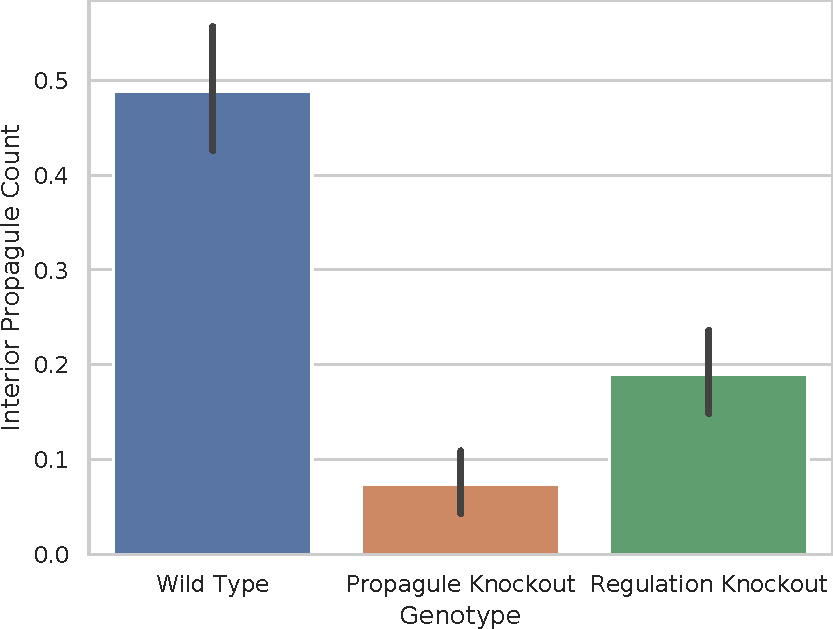
\includegraphics[width=\linewidth]{knockout/interior_propagule/title=interior_propagules+_data_hathash_hash=bb0fa6254f1b7398+_script_fullcat_hash=f738b363bea8c98a+_source_hash=53a2252-clean+ext=}%
\caption{Interior propagule rate by genotype}
\label{fig:interior_propagule_rate}
\end{subfigure}
\end{minipage}%
\hspace*{\fill}


\caption{
Analysis of a wild type strain evolved under the ``Nested-Wave'' treatment exhibiting interior propagule generation, comparing against knockouts of gene regulation and explicitly propagule-generating reproduction instructions.
Figure \ref{fig:wt_timelapse} traces the wild type life history.
Level-one groups are by differentiated by grayscale tone and separated by solid black borders.
Level-zero groups are by separated by dashed gray borders.
In each example, the focal parent level-one group is colored purple and the focal offspring group orange.
Figure \ref{fig:regulation_visualizations} depicts gene regulation at each of a cell's four directional SignalGP instances using a PCA mapping from regulatory state to three-dimensional RGB coordinates, calculated uniquely for each level-one same-channel signaling group.
Black borders divide level-one same-channel signaling groups and white borders divide level-zero same-channel signaling groups.
Endogenous daughter groups annotated with yellow arrows.
Figure \ref{fig:interior_propagule_rate} compares the mean number of interior propagules observed per level-one same-channel signaling group.
Error bars indicate 95\% confidence.
View an animation of wild type gene regulation at \url{https://mmore500.com/hopto/t}.
View the wild type strain in a live in-browser simulation at \url{https://mmore500.com/hopto/g}.
}
\label{fig:ko-interior_propagule}
\end{center}
\end{figure}


\subsection{Case Study: Intra-group Messaging}

\begin{figure*}[!htbp]
\begin{center}

\begin{minipage}[t]{\columnwidth}
\hspace*{\fill}%
\begin{minipage}[t]{0.05\columnwidth}
\vspace{0pt} % for alignment
\rotatebox{90}{Messaging}%
\end{minipage}%
\hfill
\begin{minipage}[t]{0.45\columnwidth}
\centering
\vspace{0pt} % for alignment
\adjincludegraphics[width=\textwidth, trim={{.0\width} {.0\width} {.5\width} {.5\width}}, clip]{knockout/intermessaging-sharing/wildtype/seed=1+title=directional_messaging_viz+treat=resource-wave__channelsense-yes__nlev-onebig+update=7172+_data_hathash_hash=f9e2a8ff33bf7745+_script_fullcat_hash=6b7e0389992dd616+_source_hash=53a2252-clean+ext=}%
\end{minipage}%
\hfill
\begin{minipage}[t]{0.45\columnwidth}
\centering
\vspace{0pt} % for alignment
\adjincludegraphics[width=\textwidth, trim={{.0\width} {.0\width} {.5\width} {.5\width}}, clip]{knockout/intermessaging-sharing/knockout/seed=1+title=directional_messaging_viz+treat=resource-wave__channelsense-yes__nlev-onebig+update=7172+_data_hathash_hash=ffdeb1c77dd012e1+_script_fullcat_hash=6b7e0389992dd616+_source_hash=53a2252-clean+ext=}%
\end{minipage}%
\hspace*{\fill}

\hspace*{\fill}%
\begin{minipage}[t]{0.05\columnwidth}
\vspace{0pt} % for alignment
\rotatebox{90}{Resource Sharing}%
\end{minipage}%
\hfill
\begin{minipage}[t]{0.45\columnwidth}
\centering
\vspace{0pt} % for alignment
\adjincludegraphics[width=\textwidth, trim={{.0\width} {.0\width} {.5\width} {.5\width}}, clip]{knockout/intermessaging-sharing/wildtype/seed=1+title=directional_sharing_viz+treat=resource-wave__channelsense-yes__nlev-onebig+update=7172+_data_hathash_hash=f9e2a8ff33bf7745+_script_fullcat_hash=3a1e851383e0ffd4+_source_hash=53a2252-clean+ext=}%
\end{minipage}%
\hfill
\begin{minipage}[t]{0.45\columnwidth}
\centering
\vspace{0pt} % for alignment
\adjincludegraphics[width=\textwidth, trim={{.0\width} {.0\width} {.5\width} {.5\width}}, clip]{knockout/intermessaging-sharing/knockout/seed=1+title=directional_sharing_viz+treat=resource-wave__channelsense-yes__nlev-onebig+update=7172+_data_hathash_hash=ffdeb1c77dd012e1+_script_fullcat_hash=3a1e851383e0ffd4+_source_hash=53a2252-clean+ext=}%
\end{minipage}%
\hspace*{\fill}

\hspace*{\fill}%
\begin{minipage}[t]{0.05\columnwidth}
\vspace{0pt} % for alignment
\rotatebox{90}{Resource Stockpile}%
\end{minipage}%
\hfill
\begin{minipage}[t]{0.45\columnwidth}
\centering
\vspace{0pt} % for alignment
\adjincludegraphics[width=\textwidth, trim={{.0\width} {.0\width} {.5\width} {.5\width}}, clip]{knockout/intermessaging-sharing/wildtype/seed=1+title=stockpile_viz+treat=resource-wave__channelsense-yes__nlev-onebig+update=7172+_data_hathash_hash=f9e2a8ff33bf7745+_script_fullcat_hash=4c8152cbf92e0da6+_source_hash=53a2252-clean+ext=}%
\end{minipage}%
\hfill
\begin{minipage}[t]{0.45\columnwidth}
\centering
\vspace{0pt} % for alignment
\adjincludegraphics[width=\textwidth, trim={{.0\width} {.0\width} {.5\width} {.5\width}}, clip]{knockout/intermessaging-sharing/knockout/seed=1+title=stockpile_viz+treat=resource-wave__channelsense-yes__nlev-onebig+update=7172+_data_hathash_hash=ffdeb1c77dd012e1+_script_fullcat_hash=4c8152cbf92e0da6+_source_hash=53a2252-clean+ext=}%
\end{minipage}%
\hspace*{\fill}

\vspace{1.0ex}

\hspace*{\fill}%
\begin{minipage}[t]{0.05\columnwidth}
\vspace{0pt} % for alignment
\end{minipage}%
\hfill
\begin{minipage}[t]{0.45\columnwidth}
\centering
\vspace{0pt} % for alignment
Wild Type
\end{minipage}%
\hfill
\begin{minipage}[t]{0.45\columnwidth}
\centering
\vspace{0pt} % for alignment
Messaging Knockout
\end{minipage}%
\hspace*{\fill}

\vspace{1.0ex}

\begin{subfigure}{\columnwidth}
  \caption{Phenotype visualizations}
\end{subfigure}

\end{minipage}%
\begin{minipage}[t]{\columnwidth}

\hspace*{\fill}%
\begin{minipage}[t]{\textwidth}
\centering
\vspace{0pt} % for alignment
\begin{subfigure}[b]{\textwidth}
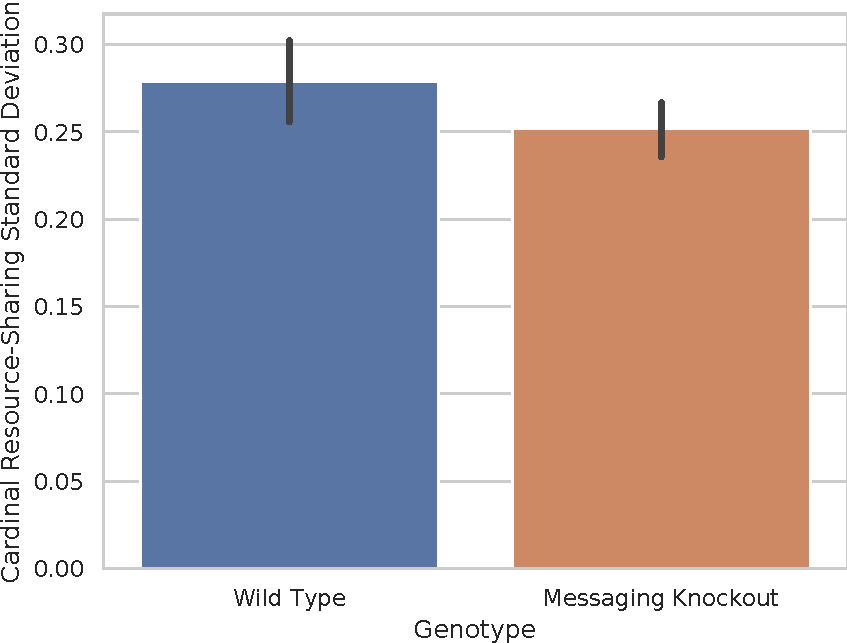
\includegraphics[width=\textwidth]{knockout/intermessaging-sharing/title=sharingdirection+_data_hathash_hash=59f6520a17fb3ad8+_script_fullcat_hash=97aad8dce5e50084+_source_hash=53a2252-clean+ext=}%
\caption{Net sharing direction variance}
\label{fig:TODO}
\end{subfigure}
\end{minipage}%
\hfill
\begin{minipage}[t]{\textwidth}
\centering
\vspace{0pt} % for alignment
\begin{subfigure}[b]{\textwidth}
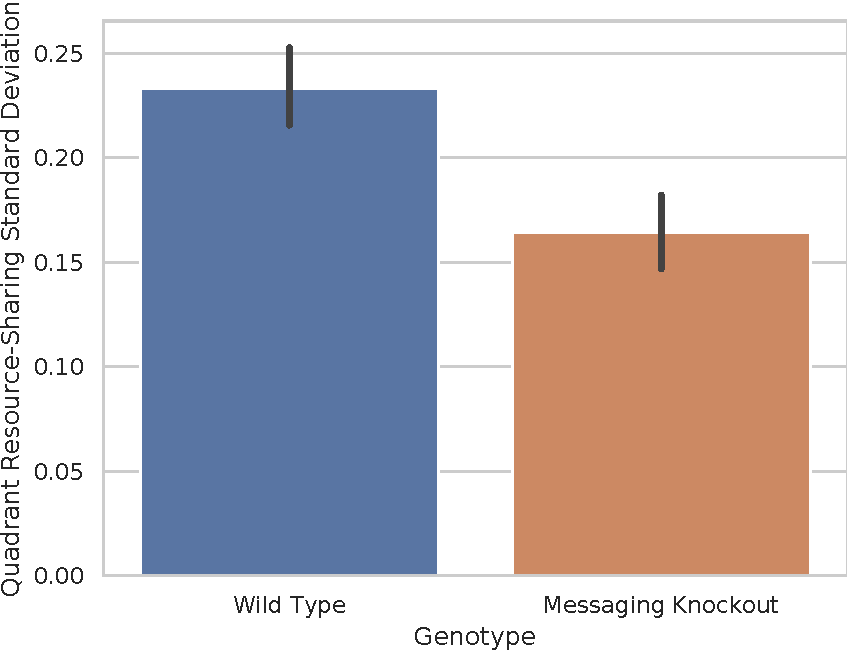
\includegraphics[width=\textwidth]{knockout/intermessaging-sharing/title=sharingquadrant+_data_hathash_hash=586f3c805332c323+_script_fullcat_hash=6e8aa37a96d9d7a9+_source_hash=53a2252-clean+ext=}%
\caption{Net sharing localization variance}
\label{fig:TODO}
\end{subfigure}
\end{minipage}%
\hfill
\begin{minipage}[t]{\textwidth}
\centering
\vspace{0pt} % for alignment
\begin{subfigure}[b]{\textwidth}
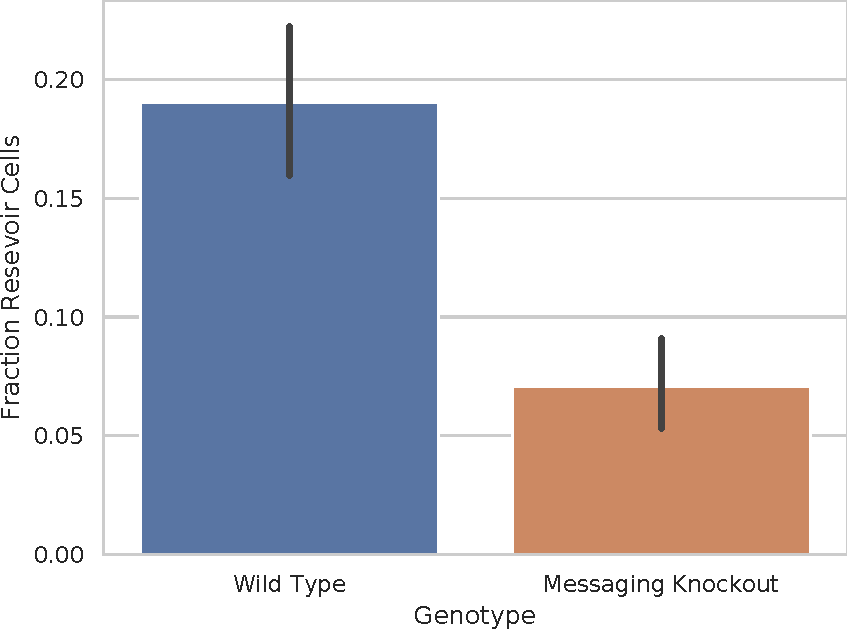
\includegraphics[width=\textwidth]{knockout/intermessaging-sharing/title=fractionresevoir+_data_hathash_hash=7ce9af7e8fe0699b+_script_fullcat_hash=da31ee3af7ae0208+_source_hash=53a2252-clean+ext=}%
\caption{Fraction of cells with enough resource to reproduce}
\label{fig:TODO}
\end{subfigure}
\end{minipage}%
\hspace*{\fill}
\end{minipage}

\caption{
TODO
}
\label{fig:ko-apoptosis}
\end{center}
\end{figure*}


\subsection{Case Study: Inter-group Messaging}

\begin{figure*}[!htbp]
\begin{center}


\begin{minipage}[t]{\columnwidth}
\centering
\hspace*{\fill}%
\begin{minipage}[t]{0.05\columnwidth}
\vspace{0pt} % for alignment
\rotatebox{90}{Messaging}%
\end{minipage}%
\hfill
\begin{minipage}[t]{0.45\columnwidth}
\centering
\vspace{0pt} % for alignment
\adjincludegraphics[width=\textwidth, trim={{.66\width} {.66\width} {.0\width} {.0\width}}, clip]{knockout/intermessaging-intergroup_border/wildtype/seed=1+title=directional_messaging_viz+treat=resource-wave__channelsense-yes__nlev-two+update=7168+_data_hathash_hash=3895dfa0dd602b4c+_script_fullcat_hash=6b7e0389992dd616+_source_hash=53a2252-clean+ext=}%
\end{minipage}%
\hfill
\begin{minipage}[t]{0.45\columnwidth}
\centering
\vspace{0pt} % for alignment
\adjincludegraphics[width=\textwidth, trim={{.66\width} {.66\width} {.0\width} {.0\width}}, clip]{knockout/intermessaging-intergroup_border/knockout/seed=1+title=directional_messaging_viz+treat=resource-wave__channelsense-yes__nlev-two+update=7168+_data_hathash_hash=24546cc614406803+_script_fullcat_hash=6b7e0389992dd616+_source_hash=53a2252-clean+ext=}%
\end{minipage}%
\hspace*{\fill}

\hspace*{\fill}%
\begin{minipage}[t]{0.05\columnwidth}
\vspace{0pt} % for alignment
\rotatebox{90}{Parent-Propagule}%
\end{minipage}%
\hfill
\begin{minipage}[t]{0.45\columnwidth}
\centering
\vspace{0pt} % for alignment
\adjincludegraphics[width=\textwidth, trim={{.66\width} {.66\width} {.0\width} {.0\width}}, clip]{knockout/intermessaging-intergroup_border/wildtype/seed=1+title=directional_propagule_viz+treat=resource-wave__channelsense-yes__nlev-two+update=7168+_data_hathash_hash=3895dfa0dd602b4c+_script_fullcat_hash=8b1f57a580a67198+_source_hash=53a2252-clean+ext=}%
\end{minipage}%
\hfill
\begin{minipage}[t]{0.45\columnwidth}
\centering
\vspace{0pt} % for alignment
\adjincludegraphics[width=\textwidth, trim={{.66\width} {.66\width} {.0\width} {.0\width}}, clip]{knockout/intermessaging-intergroup_border/knockout/seed=1+title=directional_propagule_viz+treat=resource-wave__channelsense-yes__nlev-two+update=7168+_data_hathash_hash=24546cc614406803+_script_fullcat_hash=8b1f57a580a67198+_source_hash=53a2252-clean+ext=}%
\end{minipage}%
\hspace*{\fill}

\hspace*{\fill}%
\begin{minipage}[t]{0.05\columnwidth}
\vspace{0pt} % for alignment
\rotatebox{90}{Resource Sharing}%
\end{minipage}%
\hfill
\begin{minipage}[t]{0.45\columnwidth}
\centering
\vspace{0pt} % for alignment
\adjincludegraphics[width=\textwidth, trim={{.66\width} {.66\width} {.0\width} {.0\width}}, clip]{knockout/intermessaging-intergroup_border/wildtype/seed=1+title=directional_sharing_viz+treat=resource-wave__channelsense-yes__nlev-two+update=7172+_data_hathash_hash=3895dfa0dd602b4c+_script_fullcat_hash=3a1e851383e0ffd4+_source_hash=53a2252-clean+ext=}%
\end{minipage}%
\hfill
\begin{minipage}[t]{0.45\columnwidth}
\centering
\vspace{0pt} % for alignment
\adjincludegraphics[width=\textwidth, trim={{.66\width} {.66\width} {.0\width} {.0\width}}, clip]{knockout/intermessaging-intergroup_border/knockout/seed=1+title=directional_sharing_viz+treat=resource-wave__channelsense-yes__nlev-two+update=7172+_data_hathash_hash=24546cc614406803+_script_fullcat_hash=3a1e851383e0ffd4+_source_hash=53a2252-clean+ext=}%
\end{minipage}%
\hspace*{\fill}

% \hspace*{\fill}%
% \begin{minipage}[t]{0.05\columnwidth}
% \vspace{0pt} % for alignment
% \rotatebox{90}{Resource Stockpile}%
% \end{minipage}%
% \hfill
% \begin{minipage}[t]{0.45\columnwidth}
% \centering
% \vspace{0pt} % for alignment
% \adjincludegraphics[width=\textwidth, trim={{.66\width} {.66\width} {.0\width} {.0\width}}, clip]{knockout/intermessaging-intergroup_border/wildtype/seed=1+title=stockpile_viz+treat=resource-wave__channelsense-yes__nlev-two+update=7168+_data_hathash_hash=3895dfa0dd602b4c+_script_fullcat_hash=4c8152cbf92e0da6+_source_hash=53a2252-clean+ext=}%
% \end{minipage}%
% \hfill
% \begin{minipage}[t]{0.45\columnwidth}
% \centering
% \vspace{0pt} % for alignment
% \adjincludegraphics[width=\textwidth, trim={{.66\width} {.66\width} {.0\width} {.0\width}}, clip]{knockout/intermessaging-intergroup_border/knockout/seed=1+title=stockpile_viz+treat=resource-wave__channelsense-yes__nlev-two+update=7168+_data_hathash_hash=24546cc614406803+_script_fullcat_hash=4c8152cbf92e0da6+_source_hash=53a2252-clean+ext=}%
% \end{minipage}%
% \hspace*{\fill}

\vspace{1.0ex}

\hspace*{\fill}%
\begin{minipage}[t]{0.05\columnwidth}
\vspace{0pt} % for alignment
\end{minipage}%
\hfill
\begin{minipage}[t]{0.45\columnwidth}
\centering
\vspace{0pt} % for alignment
Wild Type
\end{minipage}%
\hfill
\begin{minipage}[t]{0.45\columnwidth}
\centering
\vspace{0pt} % for alignment
Messaging Knockout
\end{minipage}%
\hspace*{\fill}

\vspace{1.0ex}

\begin{subfigure}{\columnwidth}
  \caption{Phenotype visualizations}
  \label{fig:intermessaging-intergroup_border-phen}
\end{subfigure}

\begin{minipage}[t]{0.8\columnwidth}
\centering
\vspace{0pt} % for alignment
\begin{subfigure}[b]{\textwidth}
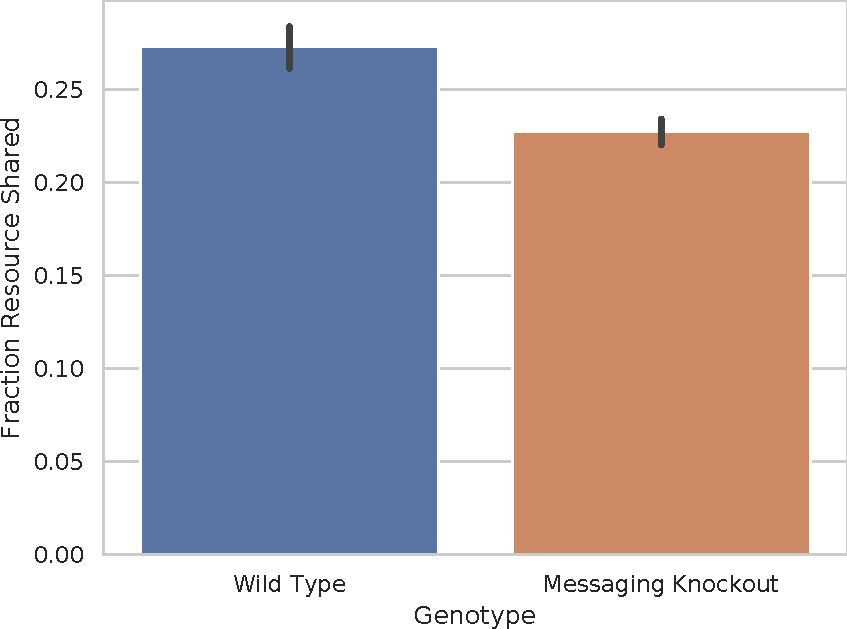
\includegraphics[width=\textwidth]{knockout/intermessaging-intergroup_border/title=sharingfraction+_data_hathash_hash=b0e9f42c3e74cf6a+_script_fullcat_hash=84ce7f4d8802dbab+_source_hash=53a2252-clean+ext=}%
\caption{Resource sharing}
\label{fig:intermessaging-intergroup_border-sharing}
\end{subfigure}
\end{minipage}%

\vspace{1ex}

\hspace*{\fill}%
\begin{minipage}[t]{0.8\columnwidth}
\centering
\vspace{0pt} % for alignment
\begin{subfigure}[b]{\textwidth}
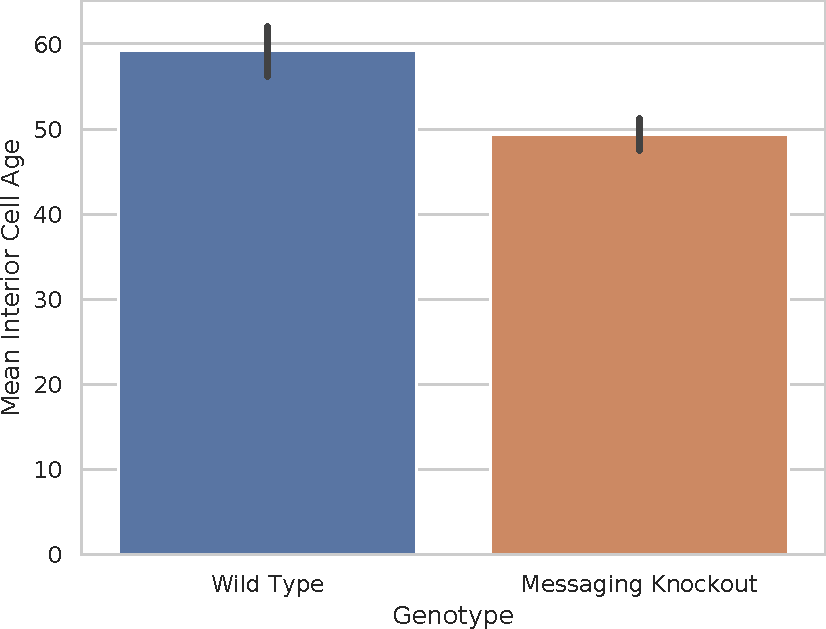
\includegraphics[width=\textwidth]{knockout/intermessaging-intergroup_border/title=cellageraw+_data_hathash_hash=ef9f5e984a40fbf6+_script_fullcat_hash=1faec38cdb6bd1de+_source_hash=53a2252-clean+ext=}%
\caption{Interior cell age}
\label{fig:intermessaging-intergroup_border-cellage}
\end{subfigure}
\end{minipage}%
\hspace*{\fill}

\end{minipage}%
\begin{minipage}[t]{\columnwidth}
\centering

\hspace*{\fill}%
\begin{minipage}[t]{0.8\columnwidth}
\centering
\vspace{0pt} % for alignment
\begin{subfigure}[b]{\textwidth}
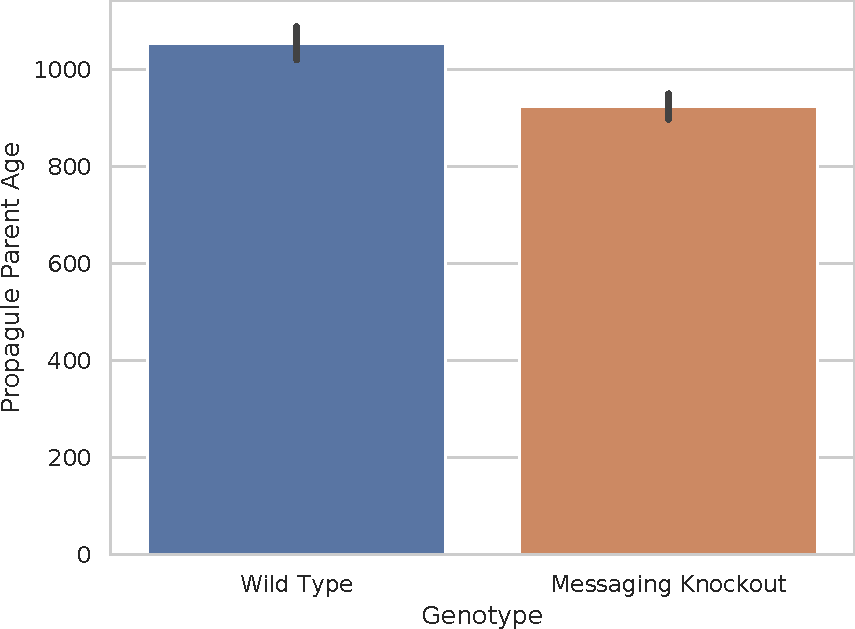
\includegraphics[width=\textwidth]{knockout/intermessaging-intergroup_border/title=parentage+_data_hathash_hash=974d02d36b7dba1a+_script_fullcat_hash=7ee3d274683ffdb2+_source_hash=53a2252-clean+ext=}%
\caption{Propagule parent age}
\label{fig:intermessaging-intergroup_border-pparentage}
\end{subfigure}
\end{minipage}%
\hspace*{\fill}

\vspace{1ex}

\hspace*{\fill}%
\begin{minipage}[t]{0.8\columnwidth}
\centering
\vspace{0pt} % for alignment
\begin{subfigure}[b]{\textwidth}
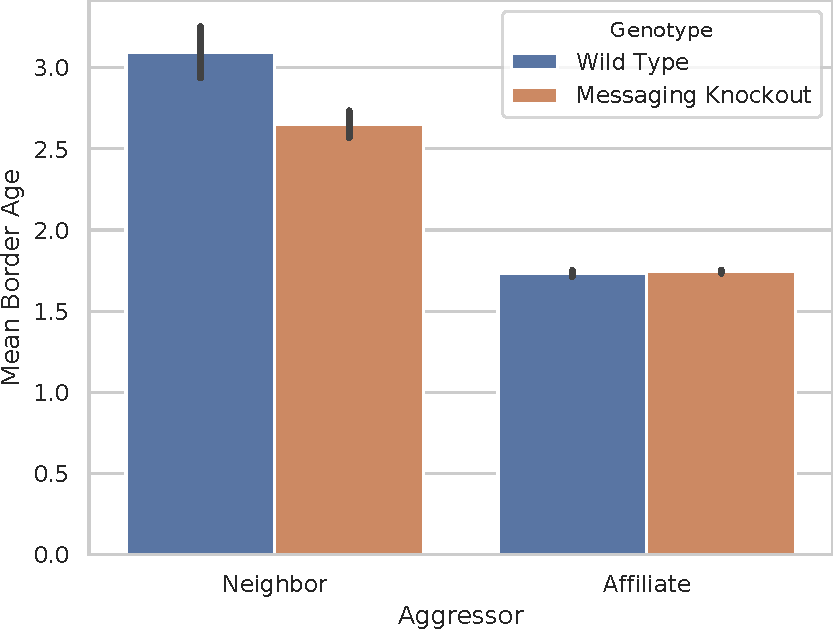
\includegraphics[width=\textwidth]{knockout/intermessaging-intergroup_border/title=comboborderage+_data_hathash_hash=8369fa84222d9217+_script_fullcat_hash=c576822d0876c8a8+_source_hash=53a2252-clean+ext=}%
\caption{Border age}
\label{fig:intermessaging-intergroup_border-borderage}
\end{subfigure}
\end{minipage}%
\hspace*{\fill}

\vspace{1ex}

\hspace*{\fill}%
\begin{minipage}[t]{0.8\columnwidth}
\centering
\vspace{0pt} % for alignment
\begin{subfigure}[b]{\textwidth}
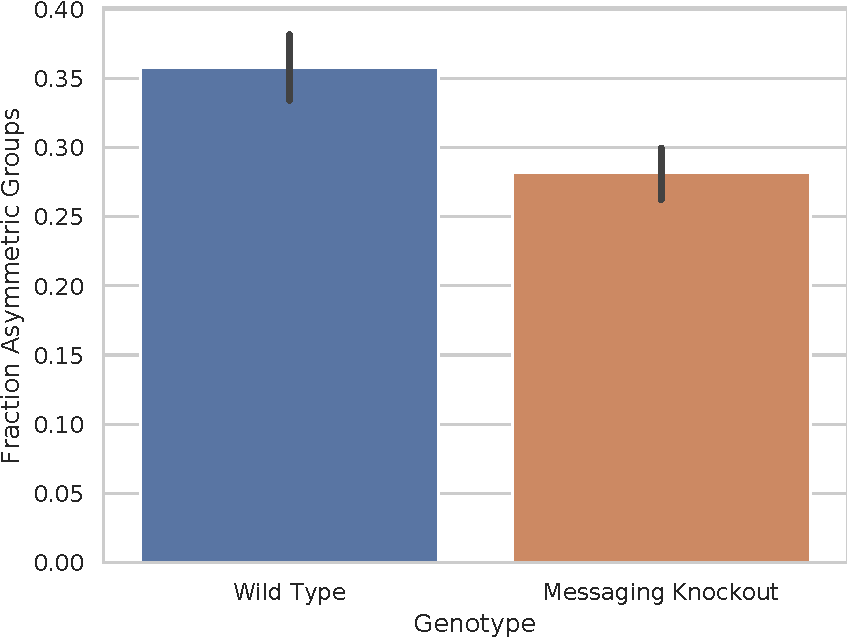
\includegraphics[width=\textwidth]{knockout/intermessaging-intergroup_border/title=metabolismasymmetry+_data_hathash_hash=3ce8f7b8474367f3+_script_fullcat_hash=0329612f3b158905+_source_hash=53a2252-clean+ext=}%
\caption{Asymmetric border metabolism}
\label{fig:intermessaging-intergroup_border-metabolism}
\end{subfigure}
\end{minipage}%
\hspace*{\fill}

\caption{
Comparison of wild type strain and corresponding intercell messaging knockout strain.
Subfigure \ref{fig:intermessaging-intergroup_border-phen} visualizes phenotypic traits in the wild type and knockout strain.
In the messaging visualization, color coding represents the volume of incoming messages.
White represents no incoming messages and the magenta to blue gradient runs from one incoming message to the maximum observed incoming message traffic.
In the resource sharing visualization, this same color coding represents the amount of incoming shared resource.
Solid black borders divide level-one same-channel signaling networks and dotted light gray borders divide level-zero same-channel signaling networks.
Subfigures \ref{fig:intermessaging-intergroup_border-sharing}, \ref{fig:intermessaging-intergroup_border-cellage}, \ref{fig:intermessaging-intergroup_border-pparentage}, \ref{fig:intermessaging-intergroup_border-borderage}, and \ref{fig:intermessaging-intergroup_border-metabolism} quantify knockout effects on various phenotypic traits.
Error bars indicate 95\% confidence.
}
\label{fig:ko-intermessaging-intergroup_border}
\end{minipage}

\end{center}
\end{figure*}


\subsection{Case Study: Gradient-Conditioned Phenotype}

\begin{figure}[!htbp]
\begin{center}

\centering

\hspace*{\fill}%
\begin{minipage}[t]{0.05\columnwidth}
\vspace{0pt} % for alignment
\rotatebox{90}{Resource Stockpile}%
\end{minipage}%
\hfill
\begin{minipage}[t]{0.45\columnwidth}
\centering
\vspace{0pt} % for alignment
\adjincludegraphics[width=\textwidth, trim={{.0\width} {.0\width} {.5\width} {.5\width}}, clip]{knockout/stockpiletrigger-sharing/wildtype/seed=1+title=stockpile_viz+treat=resource-wave__channelsense-yes__nlev-two+update=7172+_data_hathash_hash=d856da4ae5863122+_script_fullcat_hash=4c8152cbf92e0da6+_source_hash=53a2252-clean+ext=}%
\end{minipage}%
\hfill
\begin{minipage}[t]{0.45\columnwidth}
\centering
\vspace{0pt} % for alignment
\adjincludegraphics[width=\textwidth, trim={{.0\width} {.0\width} {.5\width} {.5\width}}, clip]{knockout/stockpiletrigger-sharing/knockout/seed=1+title=stockpile_viz+treat=resource-wave__channelsense-yes__nlev-two+update=7172+_data_hathash_hash=6ab6ade50c5344bc+_script_fullcat_hash=4c8152cbf92e0da6+_source_hash=53a2252-clean+ext=}%
\end{minipage}%
\hspace*{\fill}


\hspace*{\fill}%
\begin{minipage}[t]{0.05\columnwidth}
\vspace{0pt} % for alignment
\rotatebox{90}{Resource Sharing}%
\end{minipage}%
\hfill
\begin{minipage}[t]{0.45\columnwidth}
\centering
\vspace{0pt} % for alignment
\adjincludegraphics[width=\textwidth, trim={{.0\width} {.0\width} {.5\width} {.5\width}}, clip]{knockout/stockpiletrigger-sharing/wildtype/seed=1+title=directional_sharing_viz+treat=resource-wave__channelsense-yes__nlev-two+update=7172+_data_hathash_hash=d856da4ae5863122+_script_fullcat_hash=3a1e851383e0ffd4+_source_hash=53a2252-clean+ext=}%
\end{minipage}%
\hfill
\begin{minipage}[t]{0.45\columnwidth}
\centering
\vspace{0pt} % for alignment
\adjincludegraphics[width=\textwidth, trim={{.0\width} {.0\width} {.5\width} {.5\width}}, clip]{knockout/stockpiletrigger-sharing/knockout/seed=1+title=directional_sharing_viz+treat=resource-wave__channelsense-yes__nlev-two+update=7172+_data_hathash_hash=6ab6ade50c5344bc+_script_fullcat_hash=3a1e851383e0ffd4+_source_hash=53a2252-clean+ext=}%
\end{minipage}%
\hspace*{\fill}

\vspace{1.0ex}

\hspace*{\fill}%
\begin{minipage}[t]{0.05\columnwidth}
\vspace{0pt} % for alignment
\end{minipage}%
\hfill
\begin{minipage}[t]{0.45\columnwidth}
\centering
\vspace{0pt} % for alignment
Wild Type
\end{minipage}%
\hfill
\begin{minipage}[t]{0.45\columnwidth}
\centering
\vspace{0pt} % for alignment
Messaging Knockout
\end{minipage}%
\hspace*{\fill}

\vspace{1.0ex}

\caption{
Visualization of phenotypic traits of a wild type strain evolved under the ``Nested-Wave''' treatment and corresponding resource-sensing knockout strain.
In the resource-sharing visualization, color coding represents the amount of incoming shared resource.
White represents no incoming messages and the magenta to blue gradient runs from one incoming message to the maximum observed incoming message traffic.
In the resource stockpile visualization, white represents zero-resource stockpiles, blue represents stockpiles with just under enough resource to reproduce, green represents stockpiles with enough resource to reproduce, and yellow represents more than enough resource to reproduce.
Black borders divide level-one same-channel signaling groups and white borders divide level-zero same-channel signaling groups.
}
\label{fig:ko-stockpiletrigger-sharing}
\end{center}
\end{figure}



\subsection{Reproductive Division of Labor}

Figure \ref{fig:reproductive_labor}

\subsection{Resource Sharing: Cooperation Between Channel-Mates}

Figure \ref{fig:resource_contributed}

\subsection{Resource Sharing: Propagule Endowment}

Welch test ($p < 0.001$)

Figure \ref{fig:endowment}


Cell-, zeroth-, and first-level individuals were all observed at the conclusion of different runs of our evolutionary simulation (mean generation 22,016; $s=3,119$).
The criteria used to discern these outcomes are described below.
Figure \ref{fig:outcome_grids} shows the level-zero and level-one signaling networks at the end of runs where cell-, zeroth-, and first-level individuality evolved, respectively.
Figure \ref{fig:grid_progression} shows a time series of signaling network snapshots in an evolutionary run where first-level individuality evolved.
Cell-level individuals appear to form with comparatively large level-zero signaling networks that are arranged into amorphous level-one signaling networks.
Zeroth-level individuals appear to form elongated cigar-shaped level-one amalgamations of diverse level-zero networks.
First-level individuals appear to form highly regular diamond-shaped level-one amalgamations of diverse level-zero networks.

Figure \ref{fig:genotypes} describes predominant genotypes observed at the end of our evolutionary simulations.
With a single exception, nearly all evolved genotypes had $A_1$ fixed at or very near $1.0$ (i.e. population mean $A_1 \geq 0.993$).
So, reproduction over cells sharing the same level-one channel was near-universally avoided;
genotypes evolved so that cell-level organisms declined to reproduce when they were located at the interior of level-one same-channel signaling networks.

However, a variety of resource-caching strategies evolved.
Most-abundant genotypes at the end of evolutionary runs included strategies where resource was primarily cached in an organism's individual stockpile (i.e. $P_{c} > P_0, P_1$), strategies where resource was primarily cached in an organism's level-zero signaling network's pool (i.e. $P_0 > P_{c}, P_1$), and strategies where resource was primarily cached in an organism's level-one signaling network's pool (i.e. $P_1 > P_{c}, P_0$).
Among 33 trials, selfish cell-level hoarders dominated at the end of two replicates, level-zero resource-sharing dominated in 16 replicates, and level-one resource sharing dominated in 15 replicates.

Given the near-ubiquitous nature of cooperation with regard to reproductive division of labor at the level-one same-channel signaling network, it was on this basis of resource caching strategy that we drew distinctions between cell-, zeroth-, and first-level individuality.
(The single predominant genotype with $A_1 = 0.91$ had $P_0 = 1.0$, so was not sharing resource on the level-one same-channel resource pool).

Next, we wanted to compare cell-, zeroth-, and first-level individuals to determine which genotype was the most fit in the DISHTINY platform environment.
We ran ecological competitions between the the dominant genotypes from the run with greatest mean $P_{c}$, the run with greatest mean $P_0$, and the run with greatest mean $P_1$.
In 22 out of 191 trials performed fixation was reached by update 1.5 million.  The cell-level individuality genotype dominated in one trial, the zeroth-level individuality genotype dominated in 12 trials, and the first-level individuality genotype dominated in 178 trials.
These results show that in the absence of mutation, first-level individuals tend to exhibit greater fitness than zeroth- and cell-th level individuals ($p < 0.0001$; RR 2.8; two-tailed exact test).

In ecological competition, however, higher-level individuals likely benefited from elimination of somatic mutation.
To assess the relative fitness of zeroth- and first-level individuals without mutation disabled, we examined the relationship between zeroth/first-level resource pooling and the rate of cellular reproduction at the end of each of the 33 replicate evolutionary trials performed.
We observed a significant negative correlation between mean $P_0$ and cellular reproduction rate ($p < 0.0001$; bootstrap test; Figure \ref{fig:mean_res_pool1_vs_net_reproduction}) and a significant positive correlation between mean $P_1$ and cellular reproduction rate ($p < 0.0001$; bootstrap test; Figure \ref{fig:mean_res_pool2_vs_net_reproduction}).
This result suggests that first-level individuals tend to collect resource more effectively than zeroth-level individuals.
We did not test correlation between $P_{c}$ and reproduction rate due to the small number of outcomes where cell-level individuality.

With the viability of cell-, zeroth-, and first-level individuality in the DISHTINY platform environment --- and the greater relative fitness of first-level individuality --- established, we were also interested in probing the strategies employed by cell-, zeroth-, and first-level individuals beyond resource caching and reproductive deferment.
To assess whether higher-level individuals employed apoptosis to mitigate somatic mutation, we examined the relationship between zeroth/first-level resource pooling and cell-level apoptosis at the conclusion of our 33 replicate evolutionary trials.
We observed a significant negative correlation between dominant genotype $P_0$ and $M_{c}$ ($p < 0.0001$; bootstrap test; Figure \ref{fig:champion_res_pool1_vs_champion_damage_suicide0}) and a significant positive correlation between dominant genotype $P_1$ and $M_{c}$ ($p < 0.0001$; bootstrap test; Figure \ref{fig:champion_res_pool2_vs_champion_damage_suicide0}).
Notably, no genotype encoding first-level individuality was observed with $M_{c} < 0.5$.
This result suggests that first-level individuals, in particular, relied on apoptosis to mitigate somatic mutation, perhaps due to their much larger scale compared to cell- and zeroth-level individuals.

To assess whether higher-level individuals provided larger resource endowments to their propagules (offspring sharing neither the level-zero nor the level-one channel ID with the parent), we examined the relationship between zeroth/first-level resource pooling and dominant genotype first-level propagule endowment at the conclusion of our 33 replicate evolutionary trials.
We observed a significant negative correlation between dominant genotype $P_0$ and $E_1$ ($p < 0.001$; bootstrap test; Figure \ref{fig:champion_res_pool1_vs_champion_endowment2}) and a significant positive correlation between dominant genotype $P_1$ and $E_1$ ($p <  0.0001$; bootstrap test; Figure \ref{fig:champion_res_pool2_vs_champion_endowment2}).
First-level individuals might provide larger endowments to propagules simply due to a greater capacity to collect resource or perhaps because of stronger selection for well-endowed offspring when competing against other first-level individuals.
